\documentclass[letter]{emulateapj}

\usepackage{aas_macros}
\usepackage[T1]{fontenc}
\usepackage{scrextend}
\usepackage{hyperref}
\usepackage{graphicx}
\usepackage{color}
\usepackage{natbib}
\usepackage{sidecap}
\usepackage{enumitem}
\usepackage{amsmath}
\usepackage{amssymb}
\usepackage{courier}
\usepackage{xfrac}

\hypersetup{
    colorlinks=true,
    linkcolor=blue,
    filecolor=magenta,      
    urlcolor=blue,
}

\setcitestyle{numbers}

\newcommand{\cobe}{\textsl{COBE}}
\newcommand{\COBE}{\textsl{COBE}}
\newcommand{\wmap}{\textsl{WMAP}}
\newcommand{\WMAP}{\textsl{WMAP}}
\newcommand{\planck}{\textsl{Planck}}
\newcommand{\Planck}{\textsl{Planck}}
\newcommand{\lcdm}{\ensuremath{\Lambda\mathrm{CDM}}}

\shorttitle{LAMBDA overview}
\shortauthors{} 

\begin{document}

\title{Legacy Archive for Microwave Background Data Analysis (LAMBDA): An Overview}

\author{G.~E.~Addison\altaffilmark{*1}, E.~R.~Switzer\altaffilmark{$\dagger$2}, M.~R.~Greason\altaffilmark{2}, T.~B.~Griswold\altaffilmark{2}, T.~Jaffe\altaffilmark{2}, N.~Miller\altaffilmark{1,2}, N.~P.~Odegard\altaffilmark{2,3}, U.~Prasad\altaffilmark{2}, and J.~L.~Weiland\altaffilmark{1}}

\altaffiltext{*}{Corresponding author; email gaddison@jhu.edu}
\altaffiltext{$\dagger$}{LAMBDA Science Lead}
\altaffiltext{1}{
Dept. of Physics \& Astronomy, The Johns Hopkins University, 3400 N. Charles St., Baltimore, MD 21218-2686, USA
}
\altaffiltext{2}{
NASA Goddard Space Flight Center, Greenbelt, MD, USA
}
\altaffiltext{3}{
ADNET Systems, Inc., Rockville, MD, USA
}

\begin{abstract}

\noindent
This is an overview of the data products and other resources available through NASA's LAMBDA site \href{https://lambda.gsfc.nasa.gov/}{https://lambda.gsfc.nasa.gov/}. An up-to-date version of this document, along with code tools actively maintained and developed by LAMBDA staff, can be found on the LAMBDA GitHub page at \href{https://github.com/nasa-lambda/lambda_overview}{https://github.com/nasa-lambda/lambda\_overview}.\\\\New data products and other updates are announced on LAMBDA's twitter account at \href{https://twitter.com/NASA_LAMBDA}{https://twitter.com/NASA\_LAMBDA}.\\\\If you have questions or suggestions relating to LAMBDA, or are interested in joining a LAMBDA advisory group, please contact us using the form here: \href{https://lambda.gsfc.nasa.gov/contact/contact.cfm}{https://lambda.gsfc.nasa.gov/contact/contact.cfm}.

\end{abstract}

\section{Introduction}

The Legacy Archive for Microwave Background Data Analysis (LAMBDA) was set up in 2002 and is part of NASA's High Energy Astrophysics Science Archive Research Center (HEASARC, \href{https://heasarc.gsfc.nasa.gov/}{https://heasarc.gsfc.nasa.gov/}). LAMBDA provides a resource for cosmology researchers, hosting data products from cosmic microwave background (CMB) measurements, and other experiments, in addition to a range of software tools, and educational material.

\section{Data Products}

LAMBDA is the primary data host for NASA's COsmic Background Explorer (\COBE) and Wilkinson Microwave Anisotropy Probe (\WMAP) CMB satellite missions. Data products from \COBE\ are available \href{https://lambda.gsfc.nasa.gov/product/cobe/}{here} and products from \WMAP\ \href{https://lambda.gsfc.nasa.gov/product/map/current/}{here}. Additionally, we host data products from current ground-based and suborbital collaborations, including experiments listed below. We provide imbedded links to each LAMBDA experiment overview page plus a citation to a recent publication; data products can be accessed through tabs on the left of the page.
\begin{itemize}
\item \href{https://lambda.gsfc.nasa.gov/product/act/}{Atacama Cosmology Telescope (ACT)}, including polarization-sensitive ACTPol data [\citenum{louis/etal:2017}]
\item \href{https://lambda.gsfc.nasa.gov/product/bicepkeck/}{BICEP1, BICEP2, and Keck Array} [\citenum{bicep2keck:2018}] 
\item \href{https://lambda.gsfc.nasa.gov/product/polarbear/}{POLARBEAR} [\citenum{polarbear:2017}]
\item \href{https://lambda.gsfc.nasa.gov/product/quiet/}{Q/U Imaging ExperimenT (QUIET)} [\citenum{quiet:2012}] 
\item \href{https://lambda.gsfc.nasa.gov/product/spider/}{SPIDER} [\citenum{nagy/etal:2017}] 
\item \href{https://lambda.gsfc.nasa.gov/product/spt/}{South Pole Telescope (SPT)}, including polarization-sensitive SPTpol data [\citenum{henning/etal:2018}] 
\end{itemize}
These data products include maps of CMB intensity and polarization fluctuations, weight or hit maps and noise simulations, as well as higher-level data products, such as likelihood code for fitting cosmological parameters. We host archival CMB data products from earlier experiments, see list at bottom of \href{https://lambda.gsfc.nasa.gov/product/}{this page}.

LAMBDA also hosts ancillary data sets of interest to the CMB community, such as measurements of {\bf diffuse Galactic emission} for CMB or intensity mapping foreground studies. These data sets are available \href{https://lambda.gsfc.nasa.gov/product/foreground/fg_diffuse.cfm}{here}.

A collection of Galactic and extragalactic {\bf compact source catalogs} from radio, microwave, and infrared frequencies is provided \href{https://lambda.gsfc.nasa.gov/product/foreground/fg_comp_source.cfm}{here}.

{\bf Catalogs of clusters} detected using the Sunyaev Zel'dovich (SZ) effect from ACT,  \planck, and SPT, SZ angular power spectrum templates, and SZ simulations, are available \href{https://lambda.gsfc.nasa.gov/product/foreground/fg_sz_cluster.cfm}{here}.

Plots of CMB temperature, polarization, and gravitational lensing power spectra from various experiments, designed for use in presentations, are provided on the LAMBDA  \href{https://lambda.gsfc.nasa.gov/graphics/}{graphics page}. A lensing bandpower plot is provided as an example in Figure~\ref{fig:bandpower}, updated with the \planck\ 2018 results [\citenum{planck/08:2018}].

\section{Software Tools}

Several tools are actively maintained or being developed by LAMBDA staff on GitHub \href{https://github.com/nasa-lambda}{here}, including:
\begin{itemize}
\item \texttt{cmb\_footprint}, a tool to visualize footprints of different sky surveys. A sample set of CMB footprints from this tool is shown in Figure~\ref{fig:footprint}. An interactive version of the tool can be accessed on the main LAMBDA page \href{https://lambda.gsfc.nasa.gov/toolbox/footprint/aladin/aladinLAMBDA.cfm}{here}.
\item \texttt{cmb\_analysis}, a set of analysis tools including code for calculating CMB power spectra and mode-mixing matrices from temperature and polarization maps with partial sky coverage
\item \texttt{cmbpol\_plotting}, data files and code for plotting and comparing CMB power spectra measurements from different experiments
\item \texttt{docker-lambda}, a Docker image file providing Python jupyter notebooks with many useful CMB utilities, including ACTPol and BICEP1 likelihood code examples
\end{itemize}

\begin{figure}[t!]
    \centering
    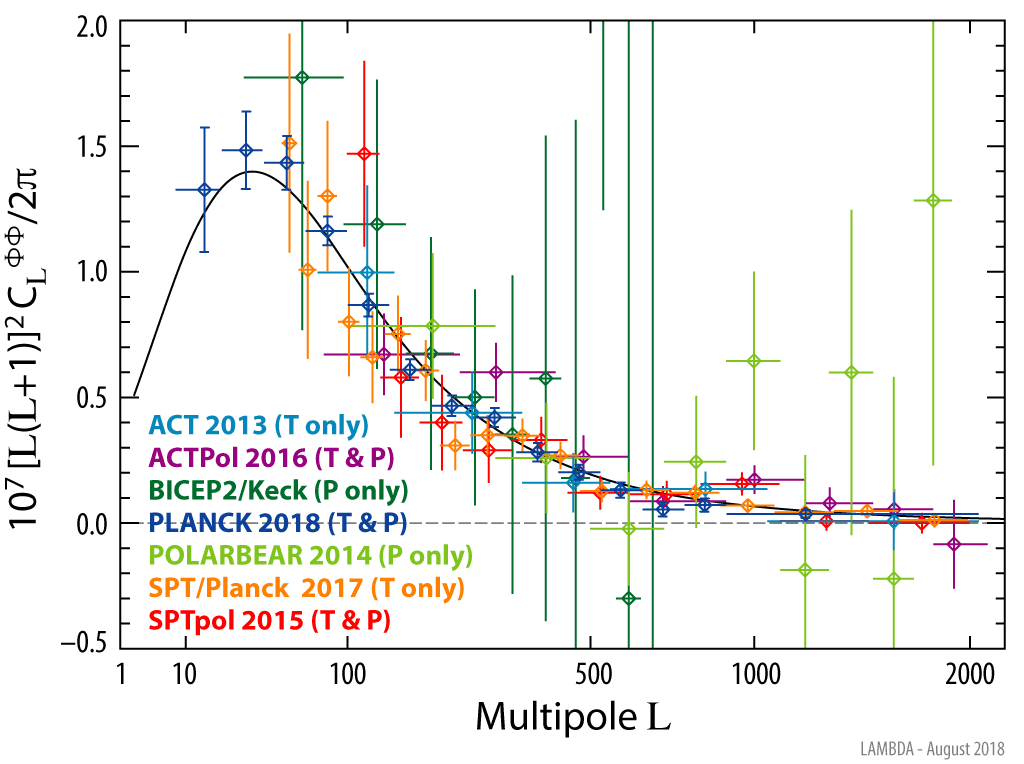
\includegraphics[width=3.464in]{fig_1}
    \caption{Compilation of CMB gravitational lensing potential power spectra from current experiments, estimated using temperature (`T') and polarization (`P') anisotropy data. This figure, and other figures comparing CMB temperature and polarization power spectra, including B-mode measurements, are available \href{https://lambda.gsfc.nasa.gov/graphics/}{here}, along with text files containing data points and error bars.}
    \label{fig:bandpower}
\end{figure}

LAMBDA also hosts an interactive version of the \texttt{CAMB} [\citenum{lewis/etal:2000}] code for generating CMB power spectra  \href{https://lambda.gsfc.nasa.gov/toolbox/tb_camb_form.cfm}{here}, and provides links to several  \href{https://lambda.gsfc.nasa.gov/toolbox/tb_converters_ov.cfm}{unit conversion utilities}, and  \href{https://lambda.gsfc.nasa.gov/toolbox/tb_calclinks.cfm}{calculator utilities}.

An extensive list of external tools for both CMB and broader astrophysical data analysis is provided with links \href{https://lambda.gsfc.nasa.gov/toolbox/}{here}. Examples include:
\begin{itemize}
    \item codes for generating CMB and matter power spectra for a given set of cosmological parameters (e.g., \texttt{CAMB}, \texttt{CLASS} [\citenum{lesgourgues:2011}], \texttt{PICO} [\citenum{fendt/wandelt:2007a}])
    \item codes for constraining cosmological parameter constraints from data using various Markov chain Monte Carlo methods (e.g., \texttt{CosmoMC} [\citenum{lewis/bridle:2002}], \texttt{MontePython} [\citenum{audren/etal:2013}])
    \item codes made public by different experimental collaborations (ACT, BICEP2/Keck, SPT, etc.) for using their data in cosmological parameter fitting (e.g., new files to use with \texttt{CosmoMC})
    \item codes for simulating aspects of the microwave sky, for example the Python Sky Model (\texttt{PySM} [\citenum{thorne/etal:2017}]), or the \texttt{Hammurabi} code for simulating polarized Galactic synchrotron emission [\citenum{waelkens/etal:2009}]
    \item tools relating to pixelization of the sky (\texttt{HEALPix}, \texttt{HEALPy} [\citenum{gorski/etal:2005}]), and calculating power spectra from pixelized sky maps (e.g., \texttt{PolSpice} [\citenum{chon/etal:2004}])
\end{itemize}

\section{Education}

LAMBDA hosts educational material, including several class and lab assignments provided by instructors, \href{https://lambda.gsfc.nasa.gov/education/}{here}. A graphical history of the \lcdm\ model, aimed at students, is provided \href{https://lambda.gsfc.nasa.gov/education/graphic_history/}{here}. This includes both theoretical material (e.g., description of components of the model and stages in evolution of the universe), and observational results, with graphical comparison of current and historical parameter constraints (e.g., age of the universe, optical depth, density of dark and baryonic matter, and Hubble constant).

\begin{figure}[h!]
    \centering
    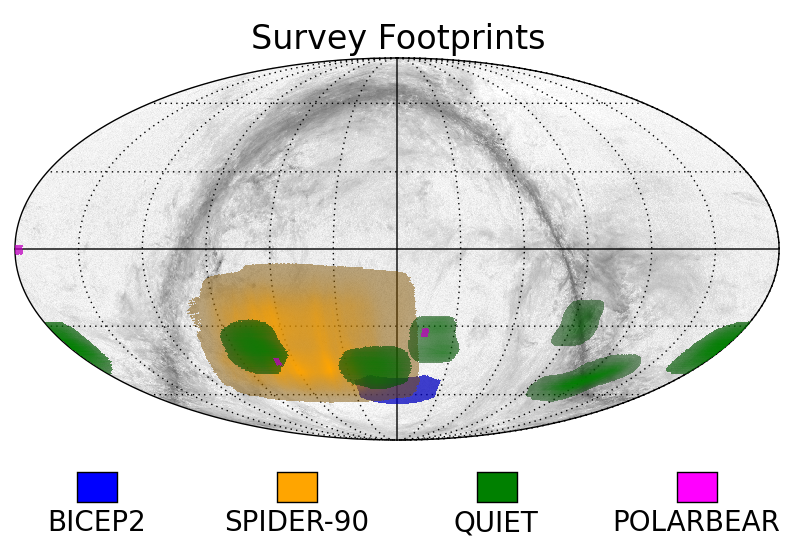
\includegraphics[width=3.464in]{fig_2.png}
    \caption{A comparison of the sky coverage of several CMB polarization surveys in equatorial coordinates, produced by the \texttt{cmb\_footprint} code. The grayscale background shows the Galactic polarized dust intensity measured by \planck.}
    \label{fig:footprint}
\end{figure}

\bibliographystyle{apj}

\begin{thebibliography}{}
\expandafter\ifx\csname natexlab\endcsname\relax\def\natexlab#1{#1}\fi

\bibitem[{{Louis} {et~al.}(2017){Louis}, {Grace}, {Hasselfield}, {Lungu},
  {Maurin}, {Addison}, {Ade}, {Aiola}, {Allison}, {Amiri}, {Angile},
  {Battaglia}, {Beall}, {de Bernardis}, {Bond}, {Britton}, {Calabrese}, {Cho},
  {Choi}, {Coughlin}, {Crichton}, {Crowley}, {Datta}, {Devlin}, {Dicker},
  {Dunkley}, {D{\"u}nner}, {Ferraro}, {Fox}, {Gallardo}, {Gralla}, {Halpern},
  {Henderson}, {Hill}, {Hilton}, {Hilton}, {Hincks}, {Hlozek}, {Ho}, {Huang},
  {Hubmayr}, {Huffenberger}, {Hughes}, {Infante}, {Irwin}, {Muya Kasanda},
  {Klein}, {Koopman}, {Kosowsky}, {Li}, {Madhavacheril}, {Marriage}, {McMahon},
  {Menanteau}, {Moodley}, {Munson}, {Naess}, {Nati}, {Newburgh}, {Nibarger},
  {Niemack}, {Nolta}, {Nu{\~n}ez}, {Page}, {Pappas}, {Partridge}, {Rojas},
  {Schaan}, {Schmitt}, {Sehgal}, {Sherwin}, {Sievers}, {Simon}, {Spergel},
  {Staggs}, {Switzer}, {Thornton}, {Trac}, {Treu}, {Tucker}, {Van Engelen},
  {Ward}, \& {Wollack}}]{louis/etal:2017}
\quad {Louis}, T., {Grace}, E., {Hasselfield}, M., {et~al.} 2017, \jcap, 6, 031

\bibitem[{{BICEP2/Keck Collaborations}(2018)}]{bicep2keck:2018}
\quad {BICEP2/Keck Collaborations}. 2018, ArXiv e-prints, arXiv:1810.05216

\bibitem[{{POLARBEAR Collaboration}(2017)}]{polarbear:2017}
\quad {POLARBEAR Collaboration}. 2017, \apj, 848, 121

\bibitem[{{QUIET Collaboration}(2012)}]{quiet:2012}
\quad {QUIET Collaboration}. 2012, \apj, 760, 145

\bibitem[{{Nagy} {et~al.}(2017){Nagy}, {Ade}, {Amiri}, {Benton}, {Bergman},
  {Bihary}, {Bock}, {Bond}, {Bryan}, {Chiang}, {Contaldi}, {Dor{\'e}},
  {Duivenvoorden}, {Eriksen}, {Farhang}, {Filippini}, {Fissel}, {Fraisse},
  {Freese}, {Galloway}, {Gambrel}, {Gandilo}, {Ganga}, {Gudmundsson},
  {Halpern}, {Hartley}, {Hasselfield}, {Hilton}, {Holmes}, {Hristov}, {Huang},
  {Irwin}, {Jones}, {Kuo}, {Kermish}, {Li}, {Mason}, {Megerian}, {Moncelsi},
  {Morford}, {Netterfield}, {Nolta}, {Padilla}, {Racine}, {Rahlin},
  {Reintsema}, {Ruhl}, {Runyan}, {Ruud}, {Shariff}, {Soler}, {Song},
  {Trangsrud}, {Tucker}, {Tucker}, {Turner}, {Van Der List}, {Weber}, {Wehus},
  {Wiebe}, \& {Young}}]{nagy/etal:2017}
\quad {Nagy}, J.~M., {Ade}, P.~A.~R., {Amiri}, M., {et~al.} 2017, \apj, 844, 151

\bibitem[{{Henning} {et~al.}(2018){Henning}, {Sayre}, {Reichardt}, {Ade},
  {Anderson}, {Austermann}, {Beall}, {Bender}, {Benson}, {Bleem}, {Carlstrom},
  {Chang}, {Chiang}, {Cho}, {Citron}, {Corbett Moran}, {Crawford}, {Crites},
  {de Haan}, {Dobbs}, {Everett}, {Gallicchio}, {George}, {Gilbert},
  {Halverson}, {Harrington}, {Hilton}, {Holder}, {Holzapfel}, {Hoover}, {Hou},
  {Hrubes}, {Huang}, {Hubmayr}, {Irwin}, {Keisler}, {Knox}, {Lee}, {Leitch},
  {Li}, {Lowitz}, {Manzotti}, {McMahon}, {Meyer}, {Mocanu}, {Montgomery},
  {Nadolski}, {Natoli}, {Nibarger}, {Novosad}, {Padin}, {Pryke}, {Ruhl},
  {Saliwanchik}, {Schaffer}, {Sievers}, {Smecher}, {Stark}, {Story}, {Tucker},
  {Vanderlinde}, {Veach}, {Vieira}, {Wang}, {Whitehorn}, {Wu}, \&
  {Yefremenko}}]{henning/etal:2018}
\quad {Henning}, J.~W., {Sayre}, J.~T., {Reichardt}, C.~L., {et~al.} 2018, \apj, 852,
  97

\bibitem[{{Planck Collaboration VIII.}(2018)}]{planck/08:2018}
\quad {Planck Collaboration VIII.} 2018, ArXiv e-prints, arXiv:1807.06210

\bibitem[{{Lewis} {et~al.}(2000){Lewis}, {Challinor}, \&
  {Lasenby}}]{lewis/etal:2000}
\quad {Lewis}, A., {Challinor}, A., \& {Lasenby}, A. 2000, \apj, 538, 473

\bibitem[{{Lesgourgues}(2011)}]{lesgourgues:2011}
\quad {Lesgourgues}, J. 2011, ArXiv e-prints, arXiv:1104.2932

\bibitem[{{Fendt} \& {Wandelt}(2007)}]{fendt/wandelt:2007a}
\quad {Fendt}, W.~A., \& {Wandelt}, B.~D. 2007, \apj, 654, 2

\bibitem[{{Lewis} \& {Bridle}(2002)}]{lewis/bridle:2002}
\quad {Lewis}, A., \& {Bridle}, S. 2002, \prd, 66, 103511

\bibitem[{{Audren} {et~al.}(2013){Audren}, {Lesgourgues}, {Benabed}, \&
  {Prunet}}]{audren/etal:2013}
\quad {Audren}, B., {Lesgourgues}, J., {Benabed}, K., \& {Prunet}, S. 2013, Journal
  of Cosmology and Astro-Particle Physics, 2013, 001

\bibitem[{{Thorne} {et~al.}(2017){Thorne}, {Dunkley}, {Alonso}, \&
  {N{\ae}ss}}]{thorne/etal:2017}
\quad {Thorne}, B., {Dunkley}, J., {Alonso}, D., \& {N{\ae}ss}, S. 2017, \mnras, 469,
  2821

\bibitem[{{Waelkens} {et~al.}(2009){Waelkens}, {Jaffe}, {Reinecke}, {Kitaura},
  \& {En{\ss}lin}}]{waelkens/etal:2009}
\quad {Waelkens}, A., {Jaffe}, T., {Reinecke}, M., {Kitaura}, F.~S., \& {En{\ss}lin},
  T.~A. 2009, \aap, 495, 697

\bibitem[{{G{\'o}rski} {et~al.}(2005){G{\'o}rski}, {Hivon}, {Banday},
  {Wandelt}, {Hansen}, {Reinecke}, \& {Bartelmann}}]{gorski/etal:2005}
\quad {G{\'o}rski}, K.~M., {Hivon}, E., {Banday}, A.~J., {et~al.} 2005, \apj, 622,
  759

\bibitem[{{Chon} {et~al.}(2004){Chon}, {Challinor}, {Prunet}, {Hivon}, \&
  {Szapudi}}]{chon/etal:2004}
\quad {Chon}, G., {Challinor}, A., {Prunet}, S., {Hivon}, E., \& {Szapudi}, I. 2004,
  \mnras, 350, 914

\end{thebibliography}

\end{document}